\section{Compare Cases}
\label{ch:comparecases}

The `Compare Cases` viewer is a standalone window for comparing several complete datasets side by side, up to six at once. It is distinct from the per-module multi-case overlay of Chapter~\ref{ch:multicase}: that workflow overlays exported CSV profiles \emph{inside} a single analysis module, whereas Compare Cases loads whole cases and compares them directly, both as 1D quantities and as full 2D fields, without re-opening each analysis module case by case.

Open the viewer from the main window. Each case is loaded independently, so cases may come from different experiments, resolutions, or grids.

\subsection{Adding cases}

\begin{quote}
\textbf{Important}
\begin{enumerate}[leftmargin=1.5em, topsep=2pt]
  \item Click `Add Case\ldots` and select the data for one case.
  \item Repeat for each case you want to compare (six maximum).
  \item Each case is given a color and a label; use the case list to rename, recolor, hide, or remove a case.
\end{enumerate}
\end{quote}

\subsection{1D comparison}

The `1D` tab overlays a chosen scalar quantity from every loaded case on a single set of axes, with a companion table listing the numeric values per case. Use the quantity selector to switch between the available 1D quantities. Because all cases share the same axes, differences in profile shape and magnitude can be read off directly.

\subsection{2D Field Compare}

The `2D Field Compare` tab shows one contour tile per case in a shared grid (up to six tiles). All tiles use a common colormap and, optionally, a common color scale, so that a given color denotes the same value in every tile. Choose the field to display (for example a velocity component or a Reynolds stress) from the field dropdown; every tile updates together.

\begin{figure}[htbp]
  \centering
  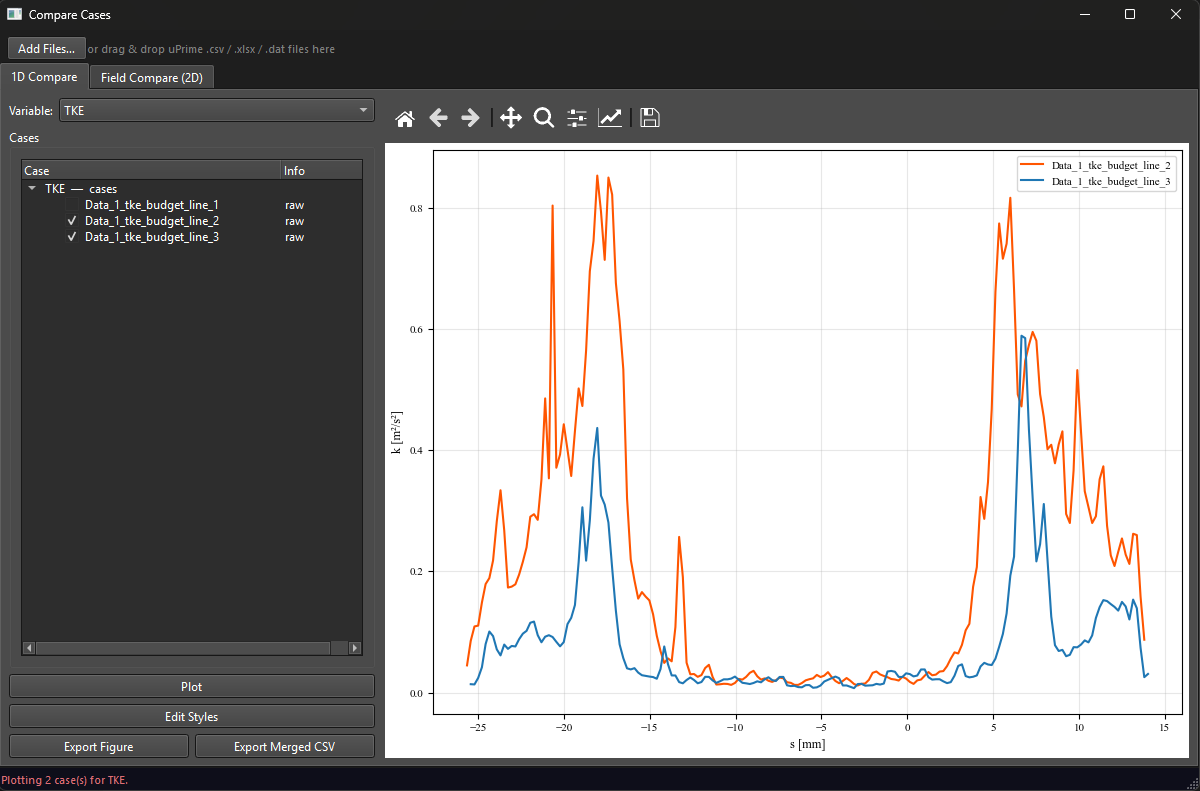
\includegraphics[width=0.92\linewidth]{fig_compare_cases}
  \caption{Compare Cases viewer, 2D Field Compare tab. Each tile is one loaded case, all sharing a common colormap and color scale so the same color denotes the same value across cases. The 1D tab (not shown) overlays a selected scalar quantity from every case on shared axes with a companion value table.}
  \label{fig:comparecases}
\end{figure}

\begin{quote}
\textbf{Tip}
For a fair visual comparison, keep the shared color scale enabled so every tile spans the same range. Disable it only when one case has a very different dynamic range and you want each tile auto-scaled to its own data.
\end{quote}

\subsection{Exporting}

Export the current comparison figure at publication resolution using the standard \href{https://cmdrryder.github.io/uPrime/}{uPrime} toolbar, following the same export conventions as the rest of the program.

% ============================= CHAPTER 16 ==============================
